\documentclass[zh,watermark]{thesis}  % draft mode (default)
%\documentclass[review]{thesis}  % review mode (show contents & reference only)
%\documentclass[watermark,final]{thesis}  % final mode (version for library)

%-------------------------------------------------------------------------------
% Package Loading
%-------------------------------------------------------------------------------

\usepackage{multirow}     % for multi-row table
\usepackage{booktabs}     % table style used in books
%\usepackage{graphviz}     % graphviz to draw graph
\usepackage{tikz}         % tikz to draw graph
\usetikzlibrary{arrows}
\usepackage{listings}

%-------------------------------------------------------------------------------
% Configuration
%-------------------------------------------------------------------------------

% 填寫題目, 作者, 指導教授, 學校, 系所, 日期等資訊
% Title
\title{Design and Implementation of a Low-Latency and High-Throughput 5G Core Network}
\titlezh{一個低延遲與高流量 5G 核心網路之設計與實作}

% Author
\authorFN{Chia-An}
\authorLN{Lee}
\authorzh{李家安}

% Advisor
\advisorFN{Jyh-Cheng}
\advisorLN{Chen}
\advisorzh{陳志成}
\advisorTitle{Dr.}
\advisorTitlezh{博士}

% First co-advisor (Leave {} empty if you don't have a co-advisor)
\coadvisorA{}
\coadvisorAzh{}
\advisorATitle{}
\advisorATitlezh{}

% Second co-advisor (Leave {} empty if you don't have a second co-advisor)
\coadvisorB{}
\coadvisorBzh{}
\advisorBTitle{}
\advisorBTitlezh{}

% Field
\field{Network Engineering}

% Institute
\institute{Institute of Computer Science and Engineering}
\institutezh{資訊科學與工程研究所}

% College
\college{College of Computer Science}

% University
\university{National Yang Ming Chiao Tung University}
\universityzh{國立陽明交通大學}

% Location
\location{Hsinchu, Taiwan, Republic of China}

% Date of final submission
\degreemonth{June}
\degreeyear{2021}
\degreeyearzh{中 華 民 國 一 百 一 十 年 六 月}

% Watermark
\watermark{figures/nctu_logo.jpg}


% 修改 thesis.cls 的預設字型
\input{config/fonts}

\begin{document}

% Show repeated author names in bibliography when using IEEEtran.bst
% Comment out this line if you don't set IEEEtran in \bibliographystyle{}
\bstctlcite{IEEEexample:BSTcontrol}

% Generate cover, title, authorization, approval and copyright pages
\maketitle

%-------------------------------------------------------------------------------
% Abstract
%-------------------------------------------------------------------------------

% 中文摘要
\begin{abstractzh}

    隨著行動網路演進至今,有越來越多功能需要滿足,第五代行動網路 (5G Cellular Networks) 也因應而生。5G 行動網路的三大訴求有
    \begin{enumerate*}
    \item 增強行動寬頻通訊 (eMBB)
    \item 超高可靠度低延遲通訊 (URLLC)
    \item 大規模物聯網通訊 (mMTC)
    \end{enumerate*},
    而藉由網路功能虛擬化的特性 (Network Function Virtualizatoin, NFV),5G 核心網路可以更加方便操作、快速佈署、無痛擴展。
    然而現如今的核心網路架構是否真的能達到上訴三大訴求?還是會為網路功能虛擬化所帶來的代價而犧牲了高流量低延遲?

    本篇論文針對高流量低延遲問題,從觀察使用情境出發,提出一套節點內降低控制端 (control plane) 通訊延遲、增加用戶端 (user plane) 通訊流量的核心網路架構並予之實作。
    在不失網路功能虛擬化特性下,透過 DPDK 與 Shared memory 的操作,小心的達到訊息溝通零記憶體複製 (zero-copy)通訊,同時對於用戶端提供規則快速查找、高流量跨節點轉發功能。

    最後針對此核心網路進行效能分析,驗證可以達到超過傳統 5G 核心網路專案 11 倍的用戶端流量與低於傳統一半的控制端延遲。

\end{abstractzh}

\keywordszh{蜂巢式網路、5G、核心網路、網路功能虛擬化}


% 英文摘要
\begin{abstract}

    As the cellular evolved, there is more and more feature must be matched in core network. That's why it comes with 5G cellular networks. In 5G, there are 3 main request:
    \begin{enumerate*}
    \item Enhanced Mobilie Broadband (eMBB)
    \item Ultra-Reliable and Low Latency Commmunications (URLLC)
    \item Massive Machine Type Communications (MMTC)
    \end{enumerate*}
    Besides, network function virtualization (NFV) are also getting more and more papular in this age. With the featues of NFV, 5G core network can be easy to operate, fast to deploye, and painless to scaled.
    However, is the architecture of 5G core network already meet the 3 requirementi nowadays? Will it suffer from high throughput and low latency only with the feature of NFV?

    This thesis with focus on the problems of high throughput and low latency. We start from some scenario observation, propose a innter-communication solution to low down the control plane communication delay and improve the user plane traffic forwarding throughput. We also implement the proof of concept to this solution and provide a new core network implementation.
    Without losing the benifit of NFV, using DPDK and shared memory, we carefully rich zero-copy control plane communication. We also provide fast rule lookup with high throughput forwarding in user plane.

    In the end, we evaluation our 5G core and proof the the user traffic can rich 11 times more efficient than origin. And the user plane latency can have one over two times then the origin one as well.

\end{abstract}

\keywordsen{Cellular Networks, 5G, Core Network, NFV}


%-------------------------------------------------------------------------------
% Acknowledgement
%-------------------------------------------------------------------------------

% 誌謝
\begin{acknowledgement}%

    % 老師
    首先我要感謝我的指導教授陳志成教授,從我還是懵董無知的專題生時,便已經給予我許多教導與建議。在就讀碩士班的兩年期間,老師不但提供了扎實的碩士訓練,讓我們從尋找問題、觀察現象、提出解決方法、驗證實作學習作研究的方法與態度,也會在我們遇到問到問題時不厭其煩的與我們討論並給予建議。同時,老師也提供了我們充足的實驗資源與設備,並透過與產業密切的合作,讓我們提早學習到產品開發過程中團隊開發、溝通合作、計劃訂定與實行的技巧。

    % 實驗室學長: Seb, Dobie, FuLian, 之前碩二, 之之前碩二, 謝哥, uDuck
    其次我要感謝 free5GC 的團隊夥伴,包含陳斯傑博士、邱德治工程師、翁甫廉工程師,以及參與開啟專案的學長姐們,包含奕華、冠穎、訓頡、家佐、張霽、啟恩、達魯學長,以及瑋庭學姊,在軟體開發初期,所有人一起討論問題、互相協助,才有 free5GC 現在的架構,在學長姐們的帶領下,我們才能比較快速的瞭解核心網路並進入開發狀態。尤其是特別感謝帶領團隊的陳斯傑學長,給予團隊正確的方向,在團隊毫無頭緒時提更我們方向,並且每每在我們對標準不甚理解時,也都能引導我們正確的瞭解標準內容。同時,我也想感謝張宏鉦研究員以及謝承穎學長,在我撰寫論文時給予許多建議與幫助,讓我在遇到問題時可以快速的找到解決方法並予之突破。

    % 實驗室同學: Jay, Yaowen, Syujy, Alan, David 學弟: Hao, Mao
    再來我想感謝的是實驗室的夥伴 彥傑、耀文、浚于、亮瑜、惟鈞,不管是課業上遇到問題時,或是計劃上碰到瓶頸,這群夥伴們都不離不棄的給予我協助、一同討論、一起面對問題。除了物理上的協助外,當我遇到挫折時,也願意聽我訴說苦水,給予我精神上的鼓勵。另外我也想感謝學弟妹們,尤其是浩澤學弟願意協助我在論文研究上的實驗,以及胤年學弟願意接手實驗室網管這項艱鉅的任務。

    % 家人
    最後我想感謝我的家人,能讓我毫無後顧之憂的學習、鑽研知識、進行研究,是家人給予我支持與鼓勵,才能讓我度過研究時遇到的種種壓力,讓我順利完成這篇論文。

\end{acknowledgement}


% 題獻頁 (Only shown in the final mode of a PhD dissertation)
\input{ack/dedication}

%-------------------------------------------------------------------------------
% 目錄
%-------------------------------------------------------------------------------

% Generate 'Table of Contents', 'List of Figures', and 'List of Tables', and
% Set page numbering to 'arabic'
\maketocs

%-------------------------------------------------------------------------------
% Contents
%-------------------------------------------------------------------------------

% Set page numbering to 'arabic' (1, 2, 3, ...)
\mainmatter

% 內文, 請依照章節順序擺放
\chapter{緒論}
\label{chapter:intro}


\section{5G 概觀}
\label{sec:5g_intro}

hihi \LaTeX

\section{研究動機與貢獻}
\label{sec:motivation_and_contribution}

% 將 free5GC 的 SMF port 到 OpenNetVM

% 提供 general 的 Golang package 讓 Go project 可以直接呼叫使用 OpenNetVM API

% 測試基於 OpenNetVM 的 AMF, SMF, 與 UPF 的效能

\chapter{背景}
\label{chapter:background}


\section{5G 核心網路簡介}
\label{sec:5g_core_intro}

\subsection{5G 核心網路用戶層介紹}
\label{subsec:5g_up_intro}

% 介紹 GTP, PFCP

\subsection{5G 核心網路控制層介紹}
\label{subsec:5g_cp_intro}

% 介紹 SBI, NGAP, NAS, PFCP

\subsection{現存 5G 核心網路專案}
\label{subsec:5g_core_project}

\section{OpenNetVM 平臺}
\label{sec:OpenNetVM}

% 其他類似平臺
% 直接用 dpdk, nff-go

\subsection{Data Plane Development Kit}
\label{subsec:DPDK}


\begin{figure}[htb]
  \centering
  % 圖片的高度與寬度, height 設為 ! 代表由寬度大小等比例縮放
  \includegraphics[height=!,width=0.6\linewidth,keepaspectratio=true]%
  % 圖片的位置
  {figures/dpdk_vs_kernel}
  % [] 放的是顯示在 list of figure 的文字
  % {} 放的是顯示在圖下方的文字
  \caption[封包處理比較:Linux 核心與 DPDK]{{\footnotesize 封包處理比較:Linux 核心與 DPDK \cite{dpdk}}}
  \label{fig:dpdk_vs_kernel}
\end{figure}

\subsection{Shared Memory}
\label{subsec:shared_memory}

\section{現行方案的挑戰}
\label{sec:challenage}

\chapter{系統架構與實作}
\label{chapter:system}


\section{實驗平台: free5GC 系統介紹}
\label{sec:free5gc_intro}

%同時介紹 free5GC control plan 採用 Golang 開發,並且介紹 Golang

free5GC 是一個現行的開源 5G 核心網路方案,在版本 v3.0.4 上原生支援 5G SA (stand-along) 架構,也就是不需要藉由 4G 網路作為中間層,包含核心網路與無線訊號接入端 (RAN, radio access network) 都可以並且必須是純 5G 之架構。而 free5GC 在 v3.0.4 上已經有實作 AMF、AUSF、NRF、NSSF、PCF、SMF、UDM、UDR、與 UPF (見圖~\ref{fig:free5gc_arch}),對於非 3GPP 接入 (non-3gpp access),free5GC 亦有 N3IWF 的支援,是目前開源 5G 核心網路方案中,架構上最爲完善的軟體。由於其開源的性質與廣大的設群討論,基於 free5GC 進行修改開發無疑是最為方便有效之選擇。

\begin{figure}[htbp]
  \centering
  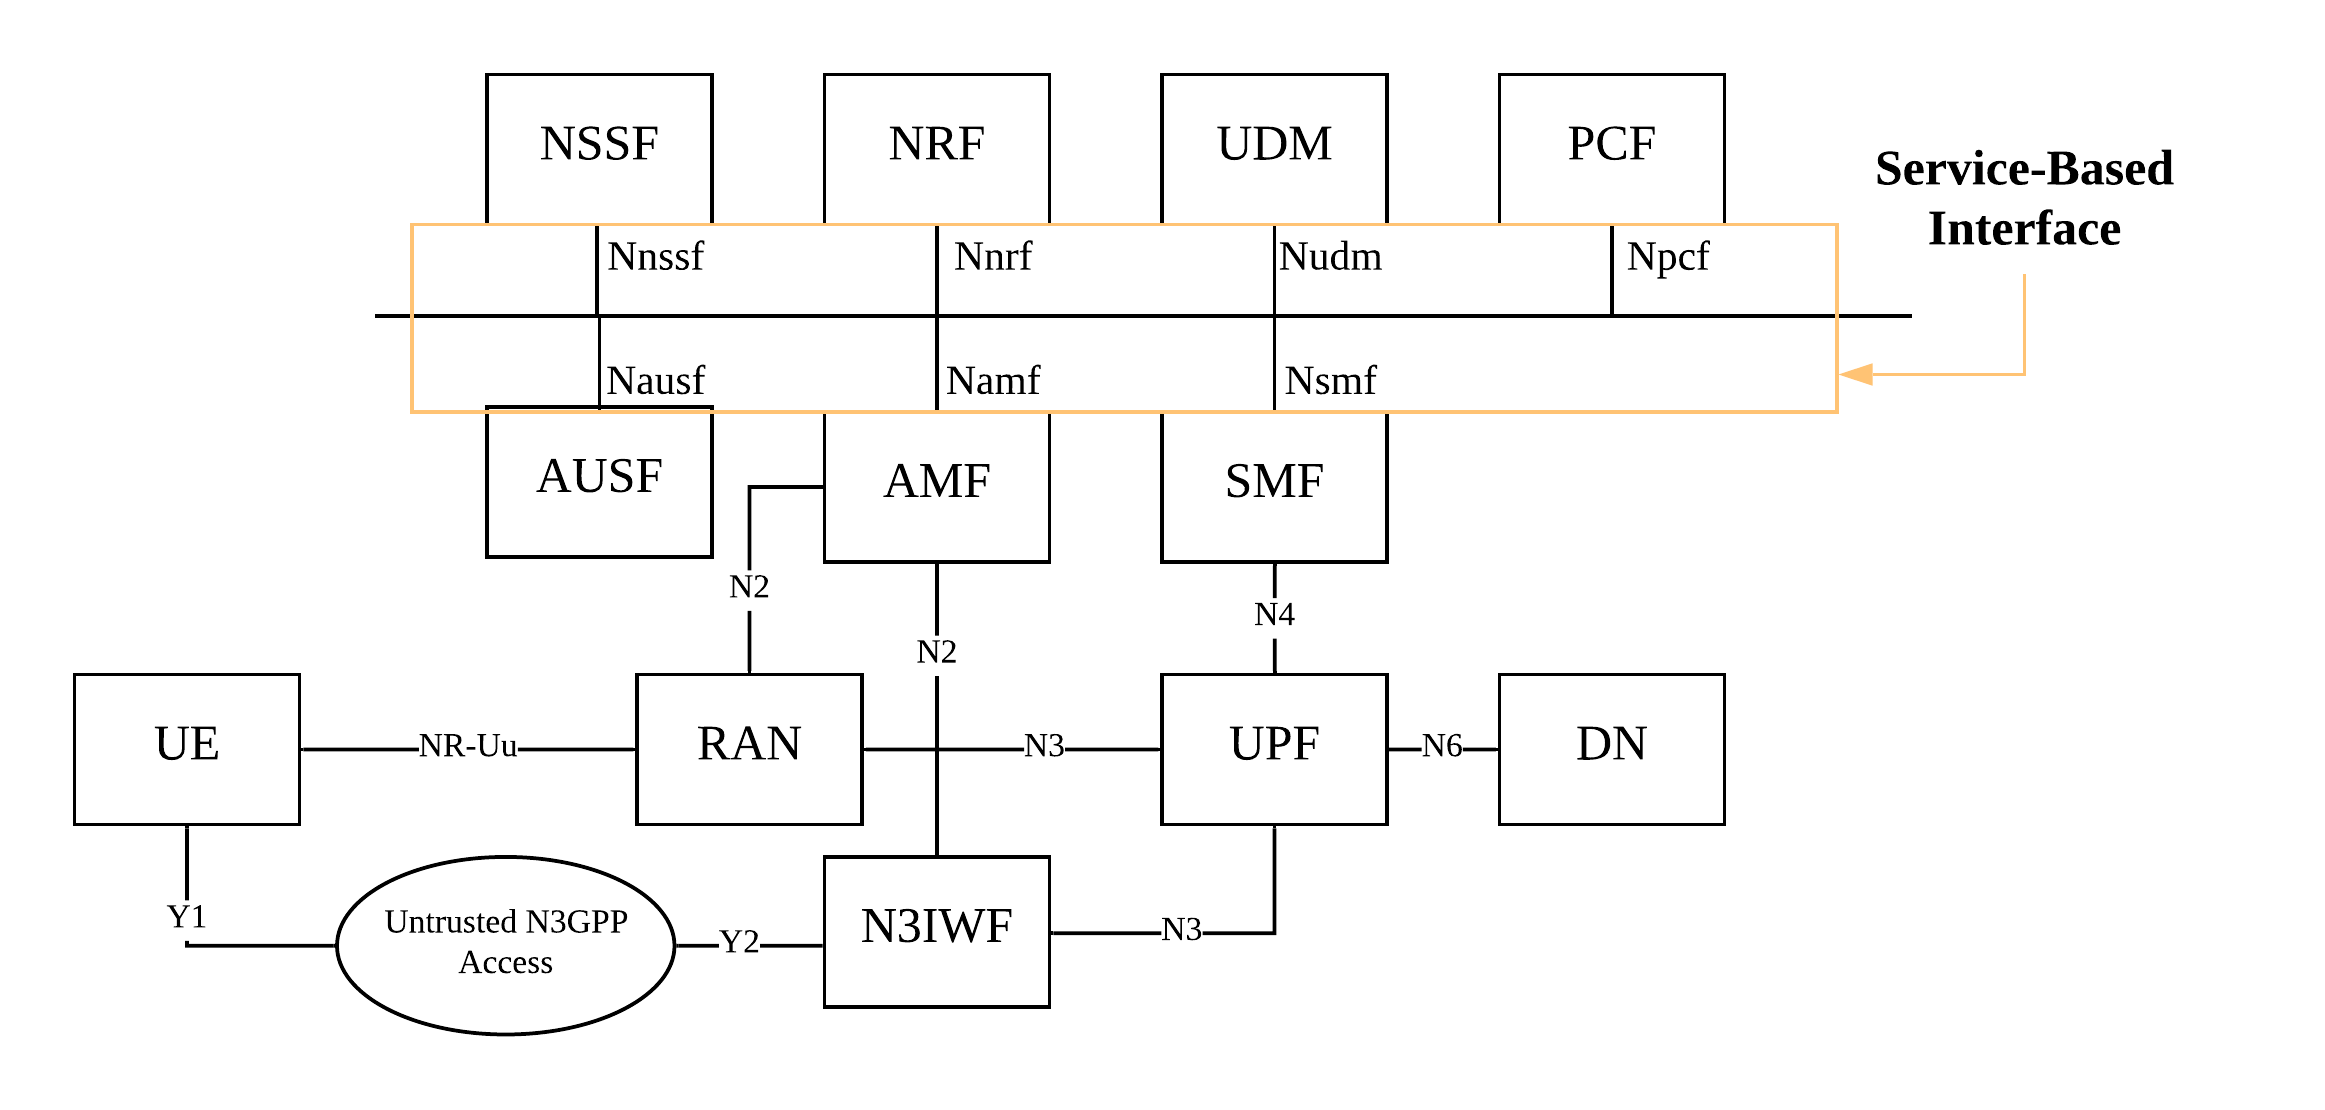
\includegraphics[height=!,width=1\linewidth,keepaspectratio=true]
                    {figures/free5gc-stage-2-arch}
  % [] 放的是顯示在 list of figure 的文字
  % {} 放的是顯示在圖下方的文字
  \caption[free5GC 架構]{{\footnotesize free5GC 架構~\cite{free5gc}}}
  \label{fig:free5gc_arch}
\end{figure}

free5GC 源自於 NextEPC~\cite{nextepc},一個 4G 開源核心網路,於版本 v1.0.0 時將 NextEPC 之 MME、S/P-GW 等運算、管理連線之 NF,改為 5G 之 AMF、SMF、與 UPF,並保留了 4G 的 HSS 與 PCRF 作認證之功能,此階段是對於 5G 架構的概念性驗證 (PoC, Proof of Concept),並沒有完全按照 3GPP 的標準實作。並且由於 NextEPC 是使用 C 語言開發,在此版本下,free5GC 亦是使用 C 語言開發,並且大量繼承使用 NextEPC 之功能與函式。

於版本 v2.0.0 時,free5GC 完全重構了核心網路,捨棄掉 NextEPC 的程式碼而改為重新開發一個基於 3GPP R15.3 的 5G 核心網路。由於考量到 Go 語言有許多適合撰寫網路程式的特性,諸如原生提供大量方便使用之標準函式庫 (standard library)、內建垃圾回收機制 (GC, garbage collection)、可快速引用第三方函式庫 (third party library) 等等,而選擇使用 Go 語言作來撰寫所有控制端 NF,唯獨 UPF 因為考量到效能以及未來可能需要與其他高效能函式庫間接的關係,而沿用 C 語言開發。

\section{系統層 API: OpenNetVM 系統介紹}
\label{sec:opennetvm_intro}

\section{系統架構總覽與目標}
\label{sec:arch_intro}

\section{SMF 移植細節}
\label{sec:smf_porting}

% 5G 所有 interface
雖然 5G 使用 SBI 架構整合了大部分的控制端界面,但還是保留了 NGAP 跟 PFCP 於 N2 及 N4 界面 (見圖~\ref{fig:5g_system_architecture}),其中 N2 是介於基地臺 (RAN) 與 AMF 之間的通訊,透過 NGAP 協定,類似於 4G 時代的 S1AP 協定,而 N4 則是 SMF 與 UPF 間的界面,沿用 4G R10 之後 CU 分離概念所使用的 PFCP 協定。在這主要的三個界面中,SBI 是基於 HTTP2,傳輸層 (L4, transport layer) 是使用的是 TCP,NGAP 的傳輸層使用 SCTP,而 PFCP 的傳輸層使用的是 UDP。

\begin{figure}[ht]
  \centering
  \subcaptionbox[b]{
    5G 系統架構,控制端用 SBI 表示
    \label{fig:5g_system_architecture_sbi}
  }{
    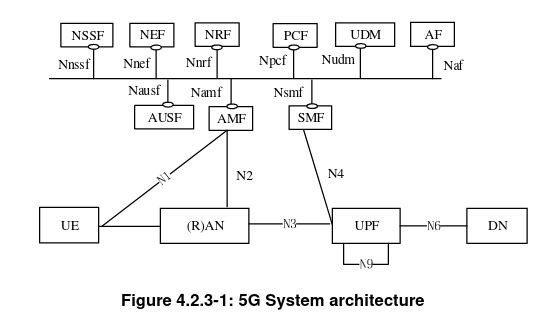
\includegraphics[height=!,width=0.45\linewidth,keepaspectratio=true]
                    {figures/23_501_4-2-3-1_sys_arch_sbi}
  }
  \subcaptionbox[b]{
    5G 系統架構,控制端用參考點表示
    \label{fig:5g_system_architecture_interface}
  }{
    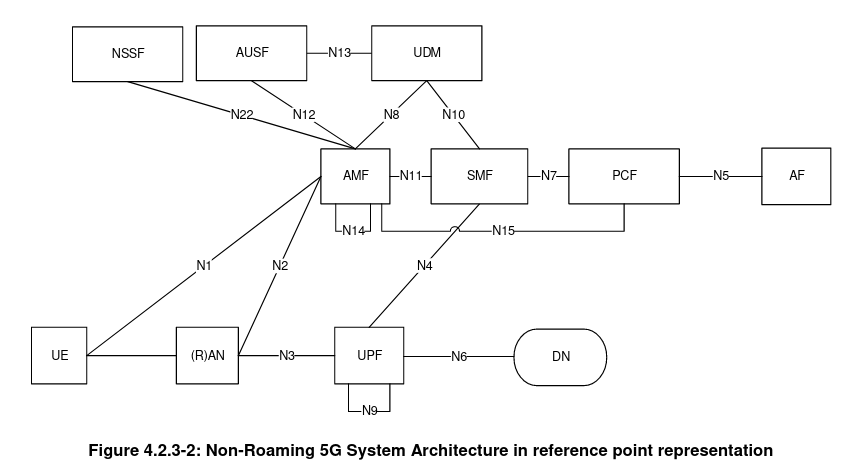
\includegraphics[height=!,width=0.45\linewidth,keepaspectratio=true]
                    {figures/23_501_4-2-3-2_sys_arch_ref}
  }
  % [] 放的是顯示在 list of figure 的文字
  % {} 放的是顯示在圖下方的文字
  \caption[5G 系統架構]{{\footnotesize 5G 系統架構~\cite{3gpp.23.501}}}
  \label{fig:5g_system_architecture}
\end{figure}

% AMF, SMF, UPF 互動內容
由於我們希望專注於改善行動網路最常見的連線行為, UE 連線上網的效能,參與這個情境需要幾乎所有 NF 的參與,但其中有三個 NF 扮演著最重要的角色,AMF、SMF、和 UPF,如同章節~\ref{sec:5g_core_intro}所描述的,AMF 主要負責處理接入 (access) 與移動 (mobility),SMF 負責連線的管理 (session management),而 UPF 則是使用者端 (user plane) 封包最重要且唯一的轉送處理單元。

連線過程主要可以分為兩個階段:註冊 (register) 與連線建立 (Session Establishment)。連線過程會做諸如確認 UE 位置、驗證使用者資料、確認使用者能力、確認一些上下文、或給予 ID 等,主要由 AMF 參與並且向其他 NF (ex. UDM, AUSF) 詢問一些資訊。而連線建立主要會幫助 UE 建立正確的連線路徑、設定 QoS 參數、設定緩衝參數等等,而在這個階段裡,除了 AMF,SMF 與 UPF 也會在這個階段內參與運算,此時 SMF 負責管理與建立連線路徑,向核心網路端他會通知 UPF 建立路徑,而向 RAN 端他會透過 AMF 的中繼 (relay),向 RAN 發出指令建立路徑或詢問資訊。

\begin{figure}[htbp]
  \centering
  \subcaptionbox[b]{
    註冊流程
    \label{fig:reg_proc}
  }{
    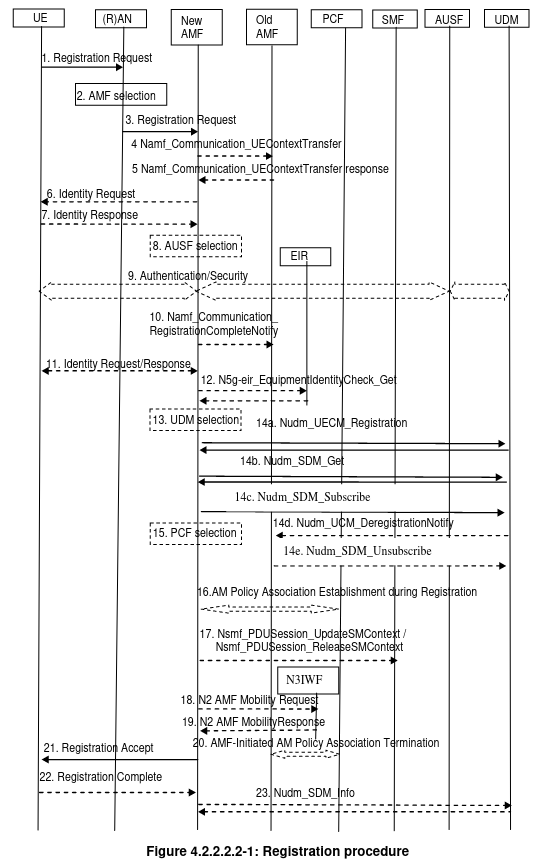
\includegraphics[height=!,width=0.4\linewidth,keepaspectratio=true]
                    {figures/23_502_4_2_2_2_2-1_reg_proc}
  }
  \subcaptionbox[b]{
    連線建立流程
    \label{fig:sess_establish}
  }{
    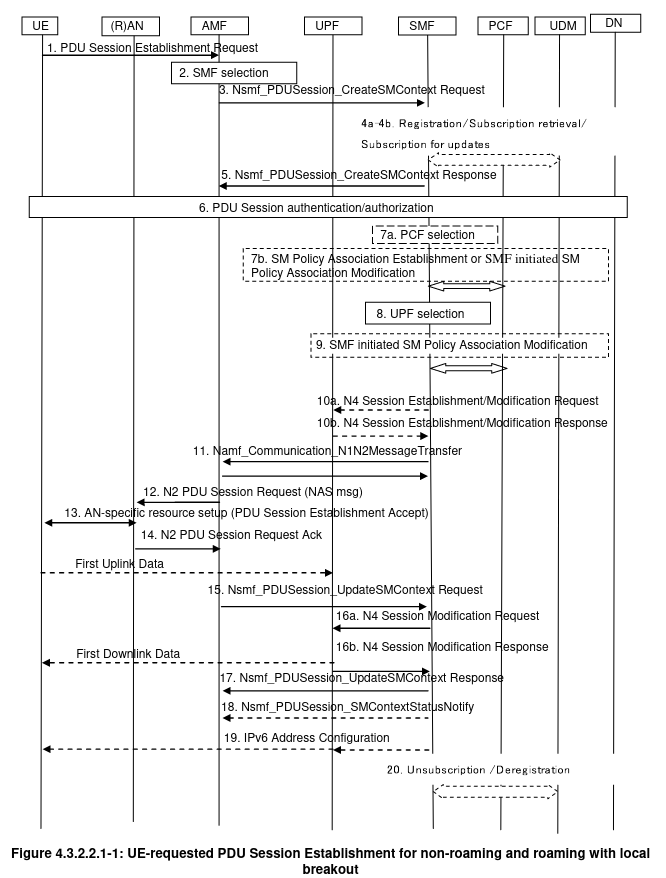
\includegraphics[height=!,width=0.475\linewidth,keepaspectratio=true]
                    {figures/23_502_4_3_2_2_1-1_sess_establish}
  }
  \caption[5G 流程]{{\footnotesize 5G 流程~\cite{3gpp.23.502}}}
  \label{fig:5g_procedure}
\end{figure}


% free5GC 原來之 SMF 架構,PFCP 使用 TLV,SBI 使用 HTTP2, OpenAPI
經過了對 free5GC 的程式碼的研讀後,我們瞭解 free5GC 大致上把控制端的 NF 大致規劃成三種部件:SBI、中心處理部件、與其他。以 SMF 為例~\ref{fig:free5gc_smf_arch},分為 SBI、Flow Procedure、與 PFCP。
SBI 全名為 service base interface
,是核心網路於 R15 (5GS) 設計出來做爲控制端溝通的協定,主要基於 HTTP2、RESTful API 設計,分為 Consumer 與 Producer,由 Consumer 向 Producer 要求 (request) 資訊。相較於 HTTP,HTTP2 提供了更少的網路延遲,而使用 RESTful API 則可讓 API 有更加的結構,並且 3GPP 直接採用 OpenAPI 格式來定義 RESTful 的格式,得以在設計好 OpenAPI 文件後,可讓人類快速讀懂,也可以透過 OpenAPI 工具直接產生出相對應的程式碼。
PFCP~\cite{3gpp.29.244} 是 SMF 獨有的協議,不存在於除 SMF 與 UPF 外的其他 NF,主要是用來讓 SMF 與 UPF 溝通,並且對 UPF 下達相對應的封包轉發指令,於 3GPP 在 R14 時為了設計 4G EPC 中 CUPS (Control and User Plane Separation, 控制與使用者端分離) 而採用的。PFCP 建立於 UDP 之上並採用 TLV (type, length, value) 的格式設計,封包內容裡每個 IE (information element) 都會有三個主要成分:2 byte 的 type 用來描述 IE 種類、2 byte 的 length 用來描述 IE value 的長度、以及 length byte 的 value 用來敘述 IE 的內容。而 TLV 亦可巢狀使用,及一個 TLV 的 value 內可以包含其他一個或多個 TLV 使用。透過 TLV 的設計,PFCP 可以將訊息有效的壓縮長度。
而 flow procedure 則是負責整個 SMF 的邏輯運算,經過 PFCP 或 SBI 解碼過的內容會被統一傳送給 Flow Procedure 並且由 Flow procedure 來決定相對要做的事情。
其他控制端 NF 架構上大致類似,若是只有 SBI 界面的 NF 像是 UDM、PCF 等等,會捨棄其他部件,而像是 AMF 有 SBI 與 NGAP,則會用 NGAP 取代其他部件。

\begin{figure}[htbp]
  \centering
  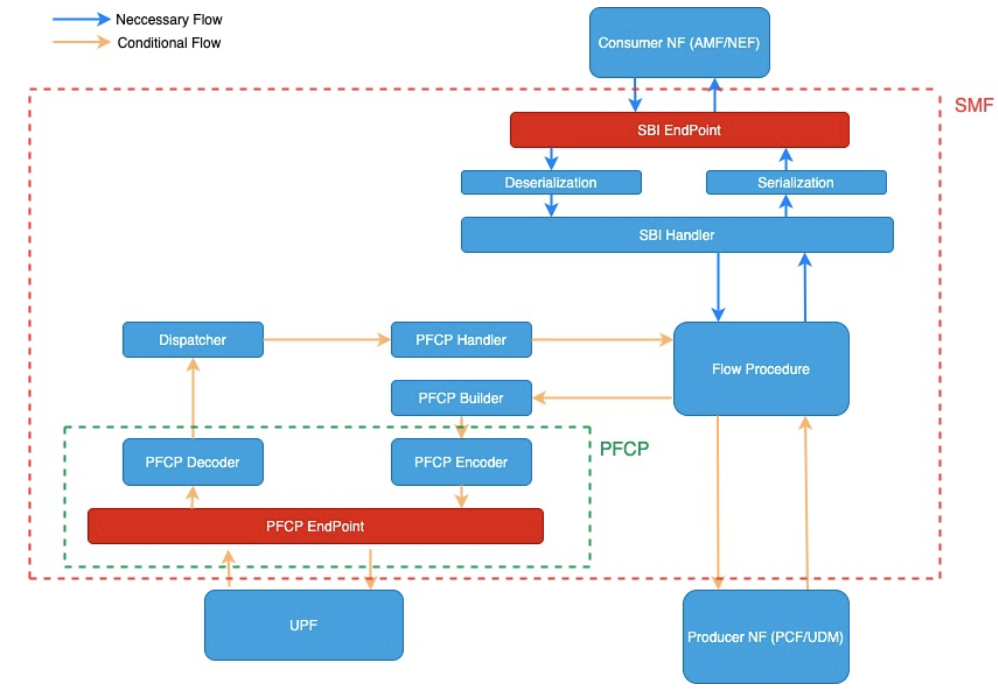
\includegraphics[height=!,width=1\linewidth,keepaspectratio=true]
                  {figures/free5gc_smf_arch}
  % [] 放的是顯示在 list of figure 的文字
  % {} 放的是顯示在圖下方的文字
  \caption[free5GC 原生之 SMF 架構]{{\footnotesize free5GC 原生之 SMF 架構}}
  \label{fig:free5gc_smf_arch}
\end{figure}

% SMF 所使用的 interface,並且決定只作 PFCP (N4 interface)
% 可以的話舉證 Session mgmt 重要於 mobility 與 regisration/deregistration
為了加速控制端的控制訊號 (control signal) 可以更快的新增、修改、刪除用戶端的會話 (session),我們希望可以透過加速 AMF、SMF、與 UPF 這三個於 PDU Session 流程中最重要的三個 Network Function 之間的通訊速度,降低其三者間的通訊延遲 (latency),得以在 5G 核心網路進行大量會話的新增、修改、與刪除中,得到最好的效能。

在 AMF、SMF、與 UPF 中,SMF 是負責 Session 管理的 Network Function,即是 Session 管理最重要的部件,因此我們希望優先著重於其控制信號的效能最佳化。而在 SMF 的界面中,又以 N4 界面用以對 UPF 下達 Session 管理的界面最為重要,因此我們決定於 N4 界面上,透過 OpenNetVM 物理層傳輸效能的優勢取代傳統 Berkeley Socket,藉以提高 N4 介面的傳輸效能,降低控制訊號的延遲。

% 移植理由, free5GC 目前的 downside (weekness)

原生的 free5GC 控制端是建構在 Linux 的 Berkeley Socket 上,先將 L4 層以上的負載內容 (payload) 封裝後,再透過呼叫 Berkeley Socket API,來達成封包傳送的功能。但由於 Berkeley Socket 屬於 user space library API,並且在傳送過程中,至少會經過兩次記憶體複製 (memory copy) (會先複製到 per process 的 kernel space memory,再複製到 network device 的 newtowrk queue) (見圖~\ref{fig:kernel_packet_processing_arch}),相對於後來出現的技術諸如 DPDK 或 XDP,實屬效能不彰。另外,即便是將 Network Function 部屬於同一機器上,由於 Berkeley Socket 屬於 RPC,傳送路徑必定會經過 Network Device,無法自動判定為 IPC 而使用更高效率的傳輸方式。基於以上理由,我們希望透過 OpenNetVM 的性質,同時可以於 RPC 下使用 DPDK 功能,與 IPC 使用 shared memory 功能,實現完全零記憶體複製 (zero copy),以及可於同一主機下使用 IPC 來達到更佳的傳輸效率。除了記憶體複製的問題之外,由於透過 system call 到 kernel 的設計,也會遇到所有 system call 會遇到的問題,像是會有至少兩種中斷 (interrupt),一個是在呼叫 system call 的中斷,另一個則是因為網卡與記憶體是透過 DMA (direct memory access) 的關係,會在 DMA 機制上需要在把封包搬進記憶體後由網卡打入中斷來呼叫中央處理器進行下一步處理。同時 kernel call 也會因為需要上下文切換 (context switch) 到中斷上下文 (interrupt context) 或甚至是遇到程序排程 (process scheduling) 的上下文切換而消耗大量運算資源與效能。

\begin{figure}[htbp]
  \centering
  \begin{tikzpicture}[semithick,scale=1]

    \draw[black, thin] (0,2) -- (16,2);
    \draw[black, thin] (0,5) -- (16,5);

    % Process
    \tikzset{process/.style = {shape=circle,draw,minimum size=1.5em}}
    \node[process] (p) at (8,6.7) {Process};
    % NIC
    \tikzset{NIC/.style = {shape=rectangle,draw,minimum size=1.5em}}
    \node[NIC] (rx) at (5,) {NIC (RX)};
    \node[NIC] (tx) at (11,) {NIC (TX)};
    % Ring
    \coordinate (rx_cod) at (5,3);
    \draw [thin] (rx_cod) circle (0.75);
    \foreach \angle in {90,67.5,...,-67.5}
        \draw ($ (\angle:0.75)+(rx_cod) $) -- ($ (\angle-180:0.75)+(rx_cod) $);
    \node [circle,thick,fill=white,draw=black,align=center] (rx_ring) at (rx_cod) {\tiny RX\\\tiny Ring};
    \coordinate (tx_cod) at (11,3);
    \draw [thin] (tx_cod) circle (0.75);
    \foreach \angle in {90,67.5,...,-67.5}
        \draw ($ (\angle:0.75)+(tx_cod) $) -- ($ (\angle-180:0.75)+(tx_cod) $);
    \node [circle,thick,fill=white,draw=black,align=center] (tx_ring) at (tx_cod) {\tiny TX\\\tiny Ring};
    % buffer
    \tikzset{buff/.style = {shape=rectangle,draw,fill=white,minimum width={width("skb")}}}
    \node[buff] (rx_skb3) at (6.65,3.88) {skb};
    \node[buff] (rx_skb2) at (6.60,3.92) {skb};
    \node[buff] (rx_skb1) at (6.55,3.94) {skb};
    \node[buff] (rx_skb) at (6.5,4) {skb};
    \node[buff] (tx_skb3) at (9.65,3.88) {skb};
    \node[buff] (tx_skb2) at (9.60,3.92) {skb};
    \node[buff] (tx_skb1) at (9.55,3.94) {skb};
    \node[buff] (tx_skb) at (9.5,4) {skb};
    \node[buff] (rx_buf) at (7,6) {recv buff};
    \node[buff] (tx_buf) at (9,6) {send buff};
    % Direction arrow
    \tikzset{copy/.style = {->,> = latex',thick,font=\scriptsize}}
    \draw[copy] (rx) .. controls (6,2) .. (rx_skb) node[pos=0.5] {copy};
    \draw[copy] (rx_skb) -- (rx_buf) node[pos=0.5] {copy};
    \draw[copy] (tx_buf) -- (tx_skb) node[pos=0.5] {copy};
    \draw[copy] (tx_skb) .. controls (10,2) .. (tx) node[pos=0.5] {copy};
    %\draw[copy] (tx_skb) to[out=225,in=135] (tx);
    % DMA & ring buffer
    \draw[double,->,> = latex] (rx) -- (rx_ring) node[pos=0.5] {DMA};
    \draw[double,->,> = latex] (tx_ring) -- (tx) node[pos=0.5] {DMA};
    \draw[dashed,->,thick] (rx_ring) -- (rx_skb);
    \draw[dashed,->,thick] (tx_ring) -- (tx_skb3);
    % text
    \node[text width=3em] at (15,6) {User Space};
    \node[text width=3em] at (15,4) {Kernel Space};
    \node[draw,text width=3em] at (13,5) {Socket};
    \node[draw,text width=3em] at (13,3.7) {Network Stack};
    \node[draw,text width=3em] at (13,2.5) {Driver};
  \end{tikzpicture}

  % [] 放的是顯示在 list of figure 的文字
  % {} 放的是顯示在圖下方的文字
  \caption[核心封包處理架構]{{\footnotesize 核心封包處理架構}}
  \label{fig:kernel_packet_processing_arch}
\end{figure}

% 開發選擇
在 SMF 移植的設計上,由於 OpenNetVM 所提供的是 C 語言的 API,而 free5GC 的 SMF 所使用的是 Golang 語言開發,因此需要考慮到如何跨語言移植。在設計之初有考慮是否需要透過 IPC 溝通,另外啟動一個 relay 將 SMF 的訊息 (message) 先透過 IPC 傳送到 relay process,再由 relay process 呼叫 OpenNetVM API。但由於發現 Golang 本身有提供 CGO 的功能,透過指定語法可以直接呼叫 C 語言 API,因此我們決定以此方法,減少 IPC 溝通的效能損耗。CGO 提供 C 呼叫 Go 語言函式或是 Go 呼叫 C 語言函式,若是以 C 呼叫 Golang,需要先將 Go 函式庫編譯成 share object library (.so 或 .dll 檔),之後再讓 C 語言透過 share object 的方式呼叫,呼叫過程中由於已經編譯成 object file 並使用 dynimic linking 的方式,是由程式跑起來後 loader 來處理,因此對 caller (C 語言程式) 幾乎沒有任何限制。反之如果是 Golang 呼叫 C 語言函式庫,則會有較多限制,例如 callee 部可以有信號 (signal) 呼叫 (基於 golang 本身訊號覆蓋(signal mask)機制)、部分型別需要做強型別轉換、需要透過 cgo flag 讓編譯器或連結器得到相對 library 絕對位置等等。

儘管透過 C program 呼叫 Golang shared library 在實踐成本上遠低於使用 Golang 呼叫 C library,但我們希望在程式設計上可以提供更高的擴充性 (scalibility) 與更加一般化 (generalize),且若可以設計成 函式庫 (library) 形式,會更加利於使用者使用且可以不僅限此專案使用,因此我們希望嘗試以可以直接使用之 Golang 函式庫方向開發。

由於從 OpenNetVM API 上獲取的封包是直接傳回封包所在記憶體位置的指標,而封包爲連結層 (link layer) 之上的內容,因此我們決定開發成類似 Goalng 原生之 net 函式庫,透過 Golang 所提供的 interface 性質,直接取代掉 PFCP 底層之 \lstinline[language=Go]{net.UdpConn} interface,我們命名之 \lstinline[language=Go]{onvmNet.ONVMConn} interface~\cite{github.onvmNet} (見圖~\ref{fig:smf_porting_arch})。

\begin{figure}[htbp]
  \centering
  \subcaptionbox{
    原生之 free5GC SMF 架構
    \label{fig:kernel_smf_arch}
  }{
    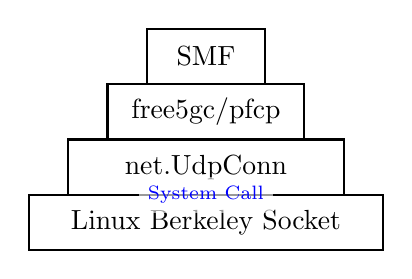
\begin{tikzpicture}
      \tikzset{
        disc 1/.style={minimum width=15mm},
        disc 2/.style={minimum width=25mm},
        disc 3/.style={minimum width=35mm},
        disc 4/.style={minimum width=45mm},
      };
      \tikzset{box/.style={minimum height=2em,draw=black,inner sep=0,thick,node distance=2em}}
      \node[disc 1,draw,box] (d1) {SMF};
      \node[disc 2,draw,box,below of=d1] (d2) {free5gc/pfcp};
      \node[disc 3,draw,box,below of=d2] (d3) {net.UdpConn};
      \node[disc 4,draw,box,below of=d3] (d4) {Linux Berkeley Socket};
      \node[below of=d3,node distance=1em,opacity=0.6,fill=white,text opacity=1,text=blue] {\scriptsize System Call};
    \end{tikzpicture}
  }
  \subcaptionbox{
    OpenNetVM 移植後之 SMF 架構
    \label{fig:onvm_smf_arch}
  }{
    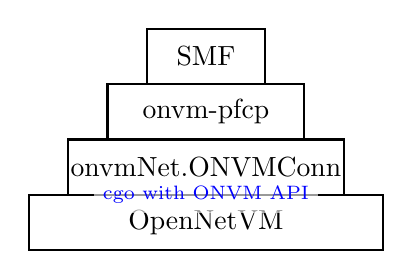
\begin{tikzpicture}
      \tikzset{
        disc 1/.style={minimum width=15mm},
        disc 2/.style={minimum width=25mm},
        disc 3/.style={minimum width=35mm},
        disc 4/.style={minimum width=45mm},
      };
      \tikzset{box/.style={minimum height=2em,draw=black,inner sep=0,thick,node distance=2em}}
      \node[disc 1,draw,box] (d1) {SMF};
      \node[disc 2,draw,box,below of=d1] (d2) {onvm-pfcp};
      \node[disc 3,draw,box,below of=d2] (d3) {onvmNet.ONVMConn};
      \node[disc 4,draw,box,below of=d3] (d4) {OpenNetVM};
      \node[below of=d3,node distance=1em,opacity=0.6,fill=white,text opacity=1,text=blue] {\scriptsize cgo with ONVM API};
    \end{tikzpicture}
  }
  % [] 放的是顯示在 list of figure 的文字
  % {} 放的是顯示在圖下方的文字
  \caption[SMF 相關性依賴]{{\footnotesize SMF 相關性依賴}}
  \label{fig:smf_porting_arch}
\end{figure}

在設計此函式庫時有部分條件需要考慮,首先,由於 Golang 在透過 CGO 呼叫 C 函式時,有不可呼叫內部有訊號註冊 (signal handling) 的函式,其原因爲 golang 本身有對訊號作內部處理,因此如果透過外部語言另外註冊訊號,會影響 Golang 程序底層訊號處理,但由於 OpenNetVM 在初始化階段需要透過 OpenNetVM 的 API 對系統作訊號註冊,因此會出現問題。而我們參考了網路上的解決方法,將訊號註冊放置 Golang 的 \lstinline[language=Go]{init} 函式,\lstinline[language=Go]{init} 函式是 Golang 設計給予在 main 函式執行起來前,就預先執行的函式,類似 C 語言的 \lstinline[language=C]{__attribute__ ((constructor))}。

然而,使用 \lstinline[language=Go]{init} 函式會遇到初始化參數無法透過程式執行過程中傳遞,因此我們採用 OpenNetVM 提供的 NF config 設計,透過 config 檔預先傳入 OpenNetVM 平臺之必要參數,諸如 DPDK 參數、Service ID、Instence ID 等。

又因為 OpenNetVM 是使用 Service ID 來決定封包目的地應該傳送至那一個 Network Function,而非使用傳統的 IP 來做 routing,因此我們也對應設計了 ipid.yaml 的檔案預先定義 IP 與 Service ID 的對應關係。透過這樣的設計,函式呼叫者 (caller) 可以直接沿用傳統 TCP 或 UDP 的呼叫,進入 onvmNet 函式之後才會透過此 ipid.yaml 檔案映射到相對應的 Service ID。

在方法 (method) 的設計上,因為我們需要繼承 \lstinline[language=Go]{net.Conn} 這個 interface,因此我們實作了此 interface 所有提供之 method,讓使用者得以直接呼叫。

另外在設計封包收取 (ReceiveFrom) 時,需要判斷此封包屬於那一個連線 (connection) 的,因此我們設計了 \lstinline{channelMap},每個連線在聽到 (listen) 連線時會開出一個對應的 channel 並放入 channelMap,當處理者 (handler) 收到 OpenNetVM 給予的封包後,透過 HashMap 的方式以 O(1) 的速度搜尋出相對應的 channel,再將封包送入 channel 得以送到正確的連線中。

% Channel dispacher 設計圖

設計完 onvmNet 函式庫後,之需將 free5GC 內部 PFCP 函式庫內有呼叫到 \lstinline[language=Go]{net.UDPConn} 的部分改成呼叫 \lstinline[language=Go]{onvmNet.ONVMConn}。另外由於 free5GC 是透過 go module 來維護套件,因此還需跟新 go.mod 之內容。而若有其他 Golang 專案想要嘗試使用 OpenNetVM 平臺,僅需作相同的取代,即可快速移植 (見圖~\ref{fig:free5gc_smf_arch})。

% ONVM SMF 總架構圖
\begin{comment}
\begin{figure}[htbp]
  \centering
  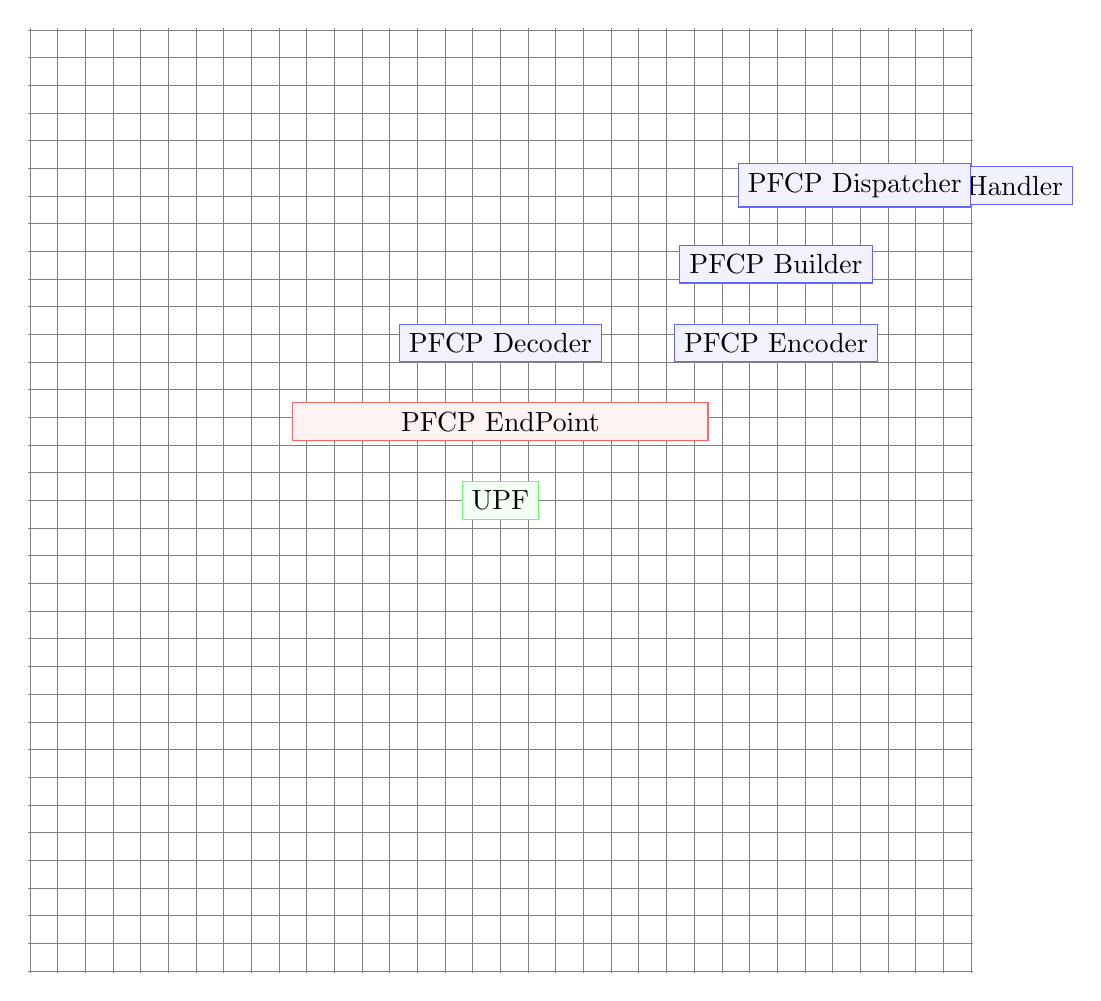
\begin{tikzpicture}
    \draw[step=1em,gray,very thin] (-6,-6) grid (6,6);
    \filldraw[black] (0,0) circle (2pt) node[anchor=west] {};

    \tikzset{
      component/.style={rectangle,draw=blue!60,fill=blue!5,thin,minimum width=7em},
      endpoint/.style={rectangle,draw=red!60,fill=red!5,thin,minimum width=15em},
      nf/.style={rectangle,draw=green!60,fill=green!5,thin},
    };
    \node[nf] (upf) {UPF};
    \node[endpoint] (pfcp_ep) [above of=upf] {PFCP EndPoint};
    \node[component] (pfcp_de) [above of=pfcp_ep] {PFCP Decoder};
    \node[component] (pfcp_en) [above of=pfcp_ep,right of=pfcp_ep,xshift=2.5cm] {PFCP Encoder};
    \node[component] (pfcp_b) [above of=pfcp_en] {PFCP Builder};
    \node[component] (pfcp_han) [above of=pfcp_b,xshift=2.5cm] {PFCP Handler};
    \node[component] (pfcp_dis) [right of=pfcp_han,xshift=-2.5cm] {PFCP Dispatcher};
  \end{tikzpicture}
\end{figure}
\end{comment}

\section{UPF 移植細節}
\label{sec:upf_porting}

\chapter{實驗與效能評估}
\label{chapter:evaluation}

為驗證本論文設計之方法,將 free5GC 核心網路移植至 OpenNetVM,使用其所提供之 ABI 能有效提升核心網路之效能,本實驗分別對原生之 free5GC 核心網路部屬於 Ubuntu Linux,與經過 OpenNetVM 移植過後之 free5GC 核心網路一樣部屬於 Ubuntu Linux,分別對其控制端(control plane)與用戶端(user plane)之效能進行測試,最終比對其結果,以驗證經過 OpenNetVM 移植過後的 free5GC 核心網路確實能有效提供更好的性能。

\section{實驗環境設定}
\label{sec:evaluation_env}

我們所使用的硬體與軟體規格如下:
\begin{itemize}
\item 中央處理器: Intel(R) Core(TM) i7-9700 CPU @ 3.00GHz
\item 處理器核心數: 8
\item 網卡: Intel Corporation Ethernet Controller X710/X557-AT 10GBASE-T 1589
\item 作業系統: centos-release-7-8.2003.0.el7.centos.x86\_64
\item 作業系統核心版本: 3.10.0-1127.el7.x86\_64
\end{itemize}

我們的實驗在邏輯上(logically)將系統分為三個部件(component),邊緣端(edge)、核心網路(core network)、與數據網路(data network)。邊緣端在真實網路下即是手機、基地臺與相關部件,以下會以 UE-RAN simulator 代稱。核心網路如第二章節所講解的,是第五代行動通訊網路中,放在機房(data center)中,負責統籌處理控制端(control plane)與轉發(forward)、封裝(encapsulate)、解封裝(decapsulate)使用者端(user plane)。而數據網路(data network),則是泛指傳統網路(the Internet),即為大多數時候,手機使用者想要存取(access)的服務之所在位置。

在務實面(physically)上將系統切分成三個節點,分別模擬使用者端發送、轉發、

為了準確的區分 traffic generating 與 forwarding 的中央處理器(以下簡稱 CPU)使用率,避免單一 CPU 需要同時產生流量與處理流量,我們的測試方法將流量產生器(traffic generator)、核心網路、流量接收者 (traffic receiver) 分別部屬於不同的機器上,讓三者得以完全妥善使用三顆不同之 CPU。

\begin{figure}[htbp]
  \centering
  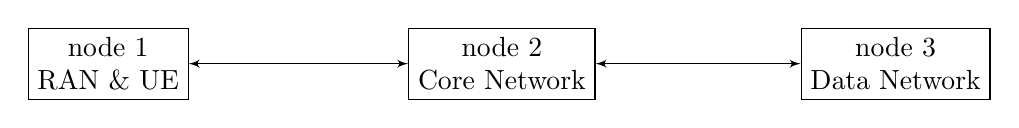
\begin{tikzpicture}

    \tikzset{vertex/.style = {shape=rectangle,draw,minimum size=1.5em,align=center}}
    \tikzset{edge/.style = {<->,> = latex'}}
    % vertices
    \node[vertex] (a) at (10,) {node 1\\RAN \& UE};
    \node[vertex] (b) at (15,) {node 2\\Core Network};
    \node[vertex] (c) at (20,) {node 3\\Data Network};
    %edges
    \draw[edge] (a) to (b);
    \draw[edge] (b) to (c);

  \end{tikzpicture}

  % [] 放的是顯示在 list of figure 的文字
  % {} 放的是顯示在圖下方的文字
  \caption[硬體架構]{{\footnotesize 硬體架構}}
  \label{fig:hardware_architecture}
\end{figure}

\section{用戶層效能分析}
\label{sec:up_evaluation}

\begin{figure}[htb]
  \centering
  % 圖片的高度與寬度, height 設為 ! 代表由寬度大小等比例縮放
  \includegraphics[height=!,width=1\linewidth,keepaspectratio=true]%
  % 圖片的位置
  {figures/user_plan_performance}
  % [] 放的是顯示在 list of figure 的文字
  % {} 放的是顯示在圖下方的文字
  \caption[用戶層效能]{{\footnotesize 用戶層效能}}
  \label{fig:user_plan_performance}
\end{figure}

\section{控制層效能分析}
\label{sec:cp_evaluation}

\chapter{結論}
\label{chapter:conclusion}

\chapter{未來展望}
\label{chapter:future}

% CGO 的 overhead 很大,也許之後可以考慮用 asm 做中間層,取代 cgo

% 自動選擇 shared memory 或 DPDK

% 完成更多 SBI 使用 shared memory

% multicore LH5GC

%\chapter{參考文獻}
\label{chapter:ref}


%-------------------------------------------------------------------------------
% 參考文獻
%-------------------------------------------------------------------------------

% Set bib style
\bibliographystyle{IEEEtran}

% Add Bibliography to "Table of Contents"
\addBibToContents

% Usage:
%   \bibliography{bib/bib1,bib/bib2,...,bib/bibN} % 注意: 不要有空格
%
% For IEEEtran users:
%   DO NOT remove bib/BSTcontrol.bib when using IEEEtran.bst. The reason is that
% when we cite two papers of the same (or similar) authors, IEEEtran.bst would
% replace the author names with "------". To avoid this, we use BSTControl.bib
% to set ctldash_repeated_names to 'no'.
%
% For non IEEEtran users:
%   Please delete bib/ieeeBSTcontrol from \bibliography{}
\bibliography{bib/ieeeBSTcontrol,bib/thesis}

%-------------------------------------------------------------------------------
% 附錄
%-------------------------------------------------------------------------------

% Start appendix
\appendix

% Add appendicies to "Table of Contents"
\addAppxToContents

% 請從此開始依序擺放附錄
%\input{appx/1-appendix}

%-------------------------------------------------------------------------------
% 作者簡歷
%-------------------------------------------------------------------------------

% 簡歷 (Only shown in a PhD dissertation)
\input{author/cv}

% 著作列表 (Only shown in a PhD dissertation)
\input{author/publications}

\end{document}
